\documentclass[letterpaper,10pt]{article}

\usepackage[T1]{fontenc}
\usepackage[utf8]{inputenc}
\usepackage[scaled]{helvet}
\renewcommand{\familydefault}{\sfdefault}
\usepackage[spanish,es-noshorthands,es-nodecimaldot]{babel}
\usepackage{icomma}
\usepackage{textcomp}
\usepackage{microtype}
\usepackage{amsmath,amssymb}
\usepackage{graphicx}
\usepackage{booktabs}
\usepackage{array}
\usepackage{enumitem}
\usepackage{titlesec}
\usepackage{fancyhdr}
\usepackage[labelsep=period,justification=centering,font=it]{caption}
\usepackage[hidelinks]{hyperref}
\usepackage[top=2.6cm,bottom=2.25cm,left=2.35cm,right=2.35cm,footskip=1.1cm]{geometry}

\graphicspath{{figuras/}}

% Numeración de secciones: "1." y "2.1."
\titleformat{\section}{\normalfont\large\bfseries}{\thesection.}{0.5em}{}
\titleformat{\subsection}{\normalfont\normalsize\bfseries}{\thesubsection.}{0.5em}{}

% Leyendas: "Fig. N." y "TABLA I."
\renewcommand{\thetable}{\Roman{table}}
\captionsetup[figure]{name=Fig.}
\captionsetup[table]{name=TABLA,font={normalfont,bf},position=top}

\setlength{\parindent}{0pt}
\setlength{\parskip}{6pt}

% Espaciado de flotantes y títulos
\setlength{\textfloatsep}{10pt plus 2pt minus 2pt}
\setlength{\intextsep}{8pt plus 2pt minus 2pt}
\setlength{\floatsep}{8pt plus 2pt minus 2pt}
\captionsetup{skip=4pt}
\renewcommand{\topfraction}{0.85}
\renewcommand{\bottomfraction}{0.7}
\renewcommand{\textfraction}{0.15}
\renewcommand{\floatpagefraction}{0.75}
\titlespacing*{\section}{0pt}{10pt plus 2pt minus 2pt}{4pt}
\titlespacing*{\subsection}{0pt}{8pt plus 2pt minus 2pt}{2pt}

\pagestyle{fancy}
\fancyhf{}
\renewcommand{\headrulewidth}{0pt}
\fancyfoot[C]{\footnotesize Universidad de los Andes | Maestría en Inteligencia Artificial \textperiodcentered{} Proyecto PDS}
\fancyfoot[R]{\footnotesize\thepage}

\begin{document}

\begin{center}
{\Large\bfseries Sistema de alertas clínicas tempranas con IA interpretable para la predicción de riesgos en niños prematuros y de bajo peso del Programa Madre Canguro\par}
\vspace{10pt}
Alex P Chirino Caicedo, Breitner E González, Santiago J Ramos Echeverry, Wilfrido A Gómez Pérez\\
Universidad de los Andes - Fundación Canguro\\
Maestría en Inteligencia Artificial, Octubre de 2026
\end{center}

\section{DESCRIPCIÓN BREVE DE LA PROPUESTA DE SOLUCIÓN}

Se desarrolló una solución de inteligencia artificial (IA) interpretable para apoyar al equipo clínico y de gestión de datos del Programa Madre Canguro \cite{charpak2005,who2022} en la revisión de registros longitudinales y la estimación de riesgos en niños prematuros o de bajo peso. La propuesta responde a dos dificultades complementarias: la calidad variable de los registros clínicos y la necesidad de anticipar desenlaces antes de la siguiente visita. El sistema no emite diagnósticos ni reemplaza la valoración profesional: organiza datos, identifica observaciones dudosas y produce estimaciones probabilísticas con explicaciones.

La solución consta de dos modelos encadenados. El primero examina la conformidad y plausibilidad de los datos mediante reglas, modelos contextuales y comparaciones longitudinales; el segundo utiliza información disponible hasta un corte de seguimiento para estimar riesgos clínicos por desenlace. El umbral que transforma un riesgo en una notificación pertenece a la aplicación y a la gobernanza clínica, no al entrenamiento del clasificador. El enfoque permite separar errores de captura de señales potencialmente clínicas y mantener trazabilidad de las decisiones.

El alcance se ajustó al comportamiento real de la fuente de datos: en lugar de reentrenamiento mensual y escritura de resultados en la base institucional, se adoptó una ejecución alineada con la carga semestral, manteniendo inferencia a demanda y separación entre datos reales y simulados. Esta decisión reduce dependencias operativas y permite evaluar el sistema con cortes reproducibles.

La solución se despliega como servicio con registro de modelos, API de inferencia y tablero web, en un entorno público con datos simulados y uno interno con los datos reales. Se discuten sus aplicaciones para priorizar el seguimiento clínico y sus límites: la pérdida de seguimiento y la deriva de la calibración.

\section{RECOLECCIÓN Y PREPARACIÓN DE LOS DATOS}

\subsection{Fuente, extracción y contrato de datos}

SEVARTI (Stages--Episodes--Variables--Topics of Interest) organiza procesos longitudinales mediante etapas de desarrollo, episodios de atención y variables vinculadas a cada momento (Fig.~\ref{fig:sevarti}). En el Programa Madre Canguro permite ubicar los controles y antecedentes en un eje de edad gestacional o corregida, diferenciando las visitas programadas de los episodios con duración propia.

\begin{figure}[!htb]
\centering
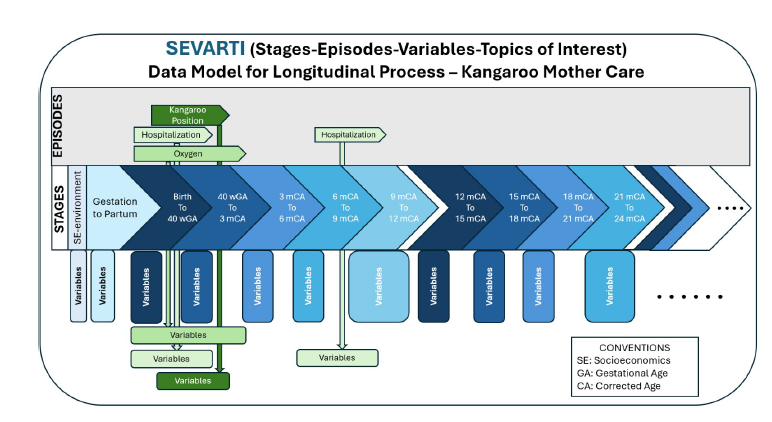
\includegraphics[width=0.55\textwidth]{fig1_sevarti.png}
\caption{Modelo conceptual SEVARTI: etapas, episodios y variables. Fuente: esquema compartido del proyecto.}
\label{fig:sevarti}
\end{figure}

Se emplearon registros de la capa de consumo de una base PostgreSQL institucional, consultada con permisos de solo lectura. El corte documentado corresponde al 24 de julio de 2026 y reúne 62.043 niños, 13.884.056 mediciones y 339 variables catalogadas (318 en uso); estas cifras describen el universo de datos del corte y no el número efectivo de observaciones de cada modelo. La extracción incorpora datos perinatales, controles antropométricos, visitas, eventos clínicos y episodios de atención. Las cifras deben asociarse siempre al corte y al criterio de conteo, pues versiones anteriores de la documentación institucional contenían 15.641 niños y aproximadamente 4,5 millones de mediciones.

El adaptador SEVARTI representa la información mediante seis entidades: esquema, etapas, sujetos, mediciones, episodios y quiebres históricos. Un diccionario administrado por expertos define variables, unidades, conceptos longitudinales, códigos de ausencia, ventanas de visita y desenlaces. Las versiones de documentación presentan diferencias en el número de variables (339--342), por lo que el conteo definitivo debe acompañarse del identificador del diccionario utilizado en cada experimento. El 76~\% de los registros carece de ubicación temporal explícita, por lo que el adaptador reconstruye el contexto con la etapa, la edad anotada y las fechas verificables.

La partición experimental se efectuó por niño y por año de nacimiento, con separación de los regímenes anteriores y posteriores al cambio de registro de 2022. Para anomalías se reportaron 40.711 niños en entrenamiento, 7.330 en calibración y 8.955 en prueba; para clasificación clínica, 48.041 en entrenamiento y 8.955 en prueba. Estas cantidades pertenecen a configuraciones experimentales distintas y no deben sumarse como si constituyeran un único particionamiento.

\subsection{Edad corregida, consistencia y tratamiento de faltantes}

La edad corregida en días se obtuvo como $\mathrm{EC} = \text{edad posnatal (días)} - 7 \times (40 - \text{edad gestacional en semanas})$. Se contrastaron fechas de nacimiento y visitas, edades consignadas, orden temporal y ventanas de seguimiento. Para el análisis de crecimiento se conservaron las edades reales de medición, dado que diferencias de semanas pueden afectar la interpretación del peso, la talla y el perímetro cefálico. Los valores dudosos se etiquetan para revisión y, según el protocolo del modelo, se excluyen como valores válidos o se tratan como faltantes; no se sustituyen automáticamente por valores estimados.

La auditoría identificó códigos de relleno no documentados en 14 variables, registros con unidades inconsistentes, fechas imposibles, medidas fuera de la ventana prevista y cambios de codificación alrededor de 2022. Se observó además pérdida de seguimiento: el registro de peso se aproxima al 78~\% en 40 semanas y al 49~\% a los 12 meses de edad corregida (Fig.~\ref{fig:cobertura}). Esta caída exige distinguir entre ausencia de dato, ausencia de visita y pérdida de seguimiento, pues la cohorte de casos completos puede no representar a todos los niños.

\begin{figure}[!htb]
\centering
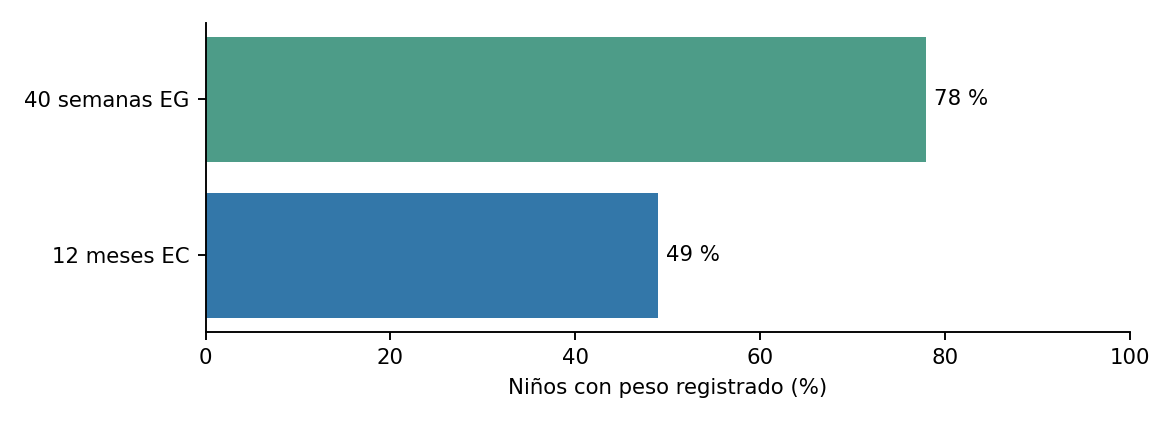
\includegraphics[width=0.62\textwidth]{fig2_cobertura_peso.png}
\caption{Cobertura de peso en dos controles, según auditoría interna del corte 24/07/2026. Gráfico elaborado para este informe a partir de porcentajes reportados.}
\label{fig:cobertura}
\end{figure}

\section{DESCRIPCIÓN DEL PROCESO DE CONSTRUCCIÓN DE LOS MODELOS O SOLUCIÓN}

\subsection{Flujo reproducible y control de versiones}

La ejecución se organiza en preparación SEVARTI, validación del diccionario, detección de anomalías, construcción de variables clínicas, entrenamiento por desenlace, evaluación y cálculo de riesgos. Cada actualización institucional puede iniciar una nueva corrida; el pipeline contempla una modalidad de evaluación silenciosa, en la cual los riesgos se guardan antes de conocer los desenlaces posteriores. Los resultados, modelos y artefactos se versionan para conservar reproducibilidad y permitir comparaciones entre cortes.

La trazabilidad del entrenamiento depende de una máscara de exclusiones versionada: se conservan los datos originales, mientras los códigos especiales, los errores de unidad y los extremos claramente inconsistentes se excluyen como objetivos de entrenamiento y se representan como faltantes en los modelos posteriores. La documentación del corte registra una exclusión del 1,6~\% de aproximadamente 3,53 millones de datos numéricos; ello no equivale a eliminar pacientes completos.

\subsection{Modelo de anomalías: cinco niveles de revisión}

Una anomalía es una observación que incumple el contrato de registro o resulta improbable por su valor, contexto clínico, trayectoria o periodo. No constituye necesariamente un error confirmado ni un diagnóstico: indica que el dato requiere revisión. Un peso plausible aisladamente, por ejemplo, puede ser incompatible con la edad corregida o con mediciones anteriores. Los cinco niveles del proceso se resumen en la Tabla~\ref{tab:niveles}.

\begin{table}[!htb]
\centering
\caption{NIVELES DE REVISIÓN DEL MODELO DE DETECCIÓN DE ANOMALÍAS}
\label{tab:niveles}
\small
\begin{tabular}{>{\raggedright\arraybackslash}p{0.18\textwidth}>{\raggedright\arraybackslash}p{0.38\textwidth}>{\raggedright\arraybackslash}p{0.36\textwidth}}
\toprule
Nivel & Procedimiento & Salida o propósito \\
\midrule
0. Contrato & Tipo, unidad, códigos y ubicación temporal & Dato válido, rechazado o no ubicable \\
1. Valor & Estadísticos robustos; detección de extremos y escala & Posibles valores anómalos o errores de unidad \\
2. Contexto & LightGBM cuantílico (Q25, Q50, Q75) y residuo calibrado & Incompatibilidad con antecedentes y visita \\
3. Trayectoria & Diferencias y velocidades entre medidas consecutivas & Saltos inesperados y secuencias incoherentes \\
4. Grupo-tiempo & Cambios trimestrales, redondeo y faltantes & Posibles cambios en prácticas de registro \\
\bottomrule
\end{tabular}
\end{table}

La revisión robusta calcula $z_r = (x - \text{mediana})/(1{,}4826 \times \mathrm{MAD})$, con MAD como mediana de desviaciones absolutas, y señala candidatos cuando $|z_r| > 3{,}5$. En la capa contextual se ajustan, por cada variable numérica, tres regresiones cuantílicas LightGBM \cite{ke2017} que estiman $Q_{0,25}$, $Q_{0,50}$ y $Q_{0,75}$ a partir de otras características del niño, la visita y el momento de medición, excluyendo el propio valor evaluado. El residuo $z_2 = (y - Q_{0,50})/[(Q_{0,75} - Q_{0,25})/1{,}349]$ se contrasta con un umbral conformal \cite{angelopoulos2023} obtenido del cuantil $1 - \alpha$ de $|z_2|$ en la partición de calibración ($\alpha = 0{,}005$); la tasa empírica de alertas puede diferir de la nominal. El entrenamiento documentado generó 132 modelos contextuales en 15,7 minutos de CPU.

La capa longitudinal contrasta cambios entre visitas con velocidades de referencia y tolerancias por concepto. La capa temporal agrega indicadores trimestrales de residuos, faltantes y redondeo, los contrasta con los ocho trimestres previos y los analiza mediante CUSUM \cite{page1954} para detectar alteraciones sistemáticas en grupos o periodos. La salida prioriza registros para revisión y proporciona motivos, no una etiqueta clínica definitiva.

\subsection{Clasificación de riesgos y explicabilidad}

Para cada desenlace y corte de seguimiento se preparan firmas con antecedentes basales, historia de visitas, episodios y mediciones conocidas hasta ese instante. Los clasificadores LightGBM \cite{ke2017} estiman probabilidades que se calibran mediante regresión isotónica \cite{zadrozny2002} con una partición temporal posterior al entrenamiento, y se comparan con una regla simple: el mismo modelo restringido a edad gestacional, peso al nacer y peso a la entrada. Las explicaciones basadas en TreeSHAP \cite{lundberg2017,lundberg2020} permiten examinar contribuciones de variables a una predicción, sin atribuirles interpretación causal. La salida incluye riesgo, percentil y contribuciones locales; la interfaz configura la política de visualización y el umbral de notificación corresponde a la aplicación y a los expertos clínicos.

Se evaluaron 14 desenlaces: cinco ventanas de readmisión, cinco de ausencia a la siguiente visita, dos evaluaciones de oxigenodependencia y dos de desarrollo psicomotor bajo. Los cuatro desenlaces de crecimiento a los 12 meses (peso, talla, peso para la talla y perímetro cefálico bajo el umbral antropométrico) son una extensión diferenciada y no forman parte de los 14 modelos evaluados. Para cada desenlace se deben fijar de manera explícita la fecha índice, el horizonte de predicción, la definición de etiqueta y los criterios de elegibilidad.

Para disminuir fuga de información, las características se restringen a los registros disponibles hasta cada visita; se descartan variables completadas retrospectivamente y los casos de inasistencia solo se etiquetan una vez cerrada la ventana de seguimiento. Las particiones por paciente y la separación cronológica evitan que información de controles futuros contamine la validación.

\subsection{Trayectorias antropométricas y firmas incrementales}

Una trayectoria antropométrica es la sucesión ordenada de peso, talla y perímetro cefálico de un niño, con sus edades reales y eventos asociados. Su análisis incluye nivel, dirección, velocidad y cambios de pendiente, preferiblemente mediante puntajes z de una referencia adecuada a sexo y edad corregida \cite{villar2015,fenton2013}. A diferencia de comparar solo dos visitas, permite reconocer desaceleraciones o recuperaciones; no obstante, la ausencia de controles y los intervalos irregulares limitan las comparaciones.

\textbf{Implementado.} Se estableció una trayectoria de ocho hitos: nacimiento, inicio de posición canguro, salida de posición canguro, 40 semanas de edad gestacional y controles de 3, 6, 9 y 12 meses de edad corregida. Los dos hitos de posición canguro se interpretan como eventos con fecha propia y no como visitas a una edad fija. En cada punto se vinculan peso, talla y perímetro cefálico cuando existen y se calculan indicadores estandarizados conforme a la referencia antropométrica clínicamente aprobada.

\textbf{Propuesto (siguiente fase).} Para predecir un desenlace a 12 meses se proyectarán firmas sucesivas en 40 semanas, 3, 6 y 9 meses EC (Tabla~\ref{tab:cortes}). Cada firma incluirá estado actual, cambios de puntaje z respecto al control anterior, velocidades normalizadas por días, variables basales y señales de calidad. La selección de variables combinará plausibilidad clínica, disponibilidad antes del corte, completitud, estabilidad temporal y ganancia predictiva frente a una línea base. Las interpolaciones entre visitas solo se usarán en análisis descriptivos o cuando se garantice que no emplean observaciones posteriores al instante de predicción.

\begin{table}[!htb]
\centering
\caption{CORTES DE SEGUIMIENTO E INFORMACIÓN DISPONIBLE PARA LA PREDICCIÓN INCREMENTAL}
\label{tab:cortes}
\small
\begin{tabular}{>{\raggedright\arraybackslash}p{0.16\textwidth}>{\raggedright\arraybackslash}p{0.48\textwidth}>{\raggedright\arraybackslash}p{0.28\textwidth}}
\toprule
Corte & Información admisible & Desenlace de evaluación \\
\midrule
40 semanas & Nacimiento, episodios neonatales y datos hasta 40 semanas & Estado a 12 meses EC \\
3 meses EC & Firma previa + mediciones y eventos hasta 3 meses & Estado a 12 meses EC \\
6 meses EC & Firma previa + cambios y eventos hasta 6 meses & Estado a 12 meses EC \\
9 meses EC & Firma previa + cambios y eventos hasta 9 meses & Estado a 12 meses EC \\
\bottomrule
\end{tabular}
\end{table}

\subsection{Arquitectura técnica y protección de datos}

\begin{figure}[!htb]
\centering
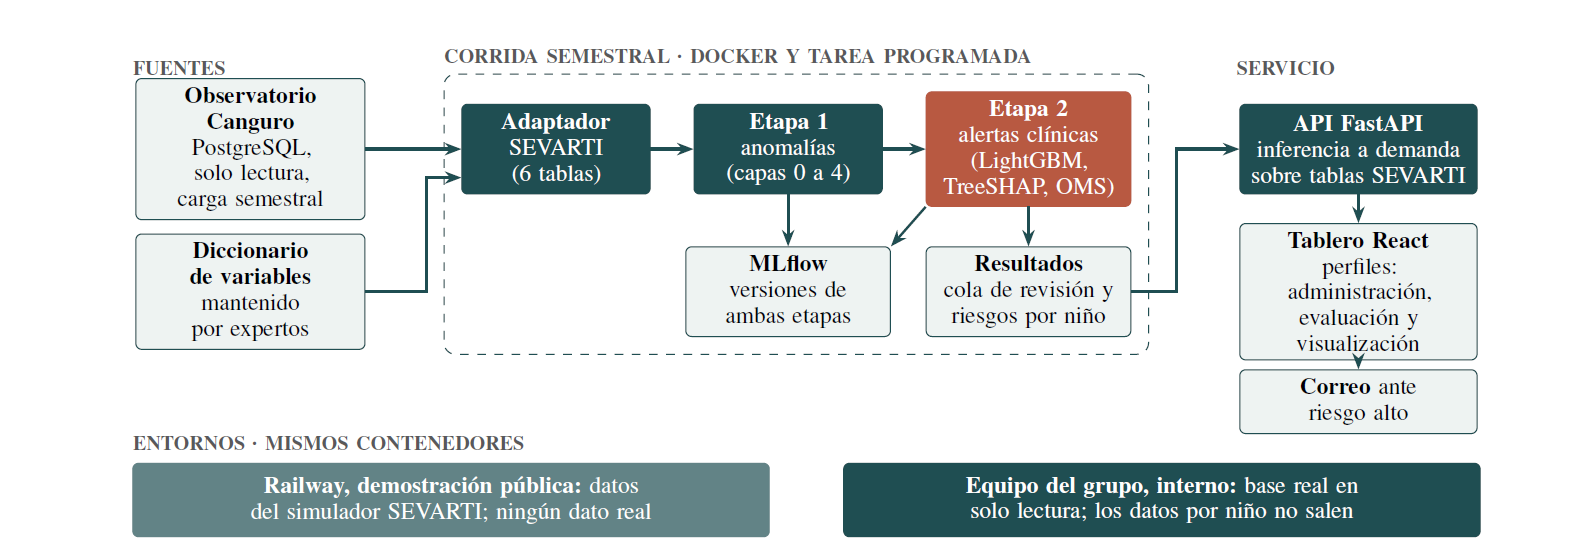
\includegraphics[width=0.88\textwidth]{fig3_arquitectura.png}
\caption{Arquitectura lógica del sistema: SEVARTI, anomalías, riesgos y servicio. La demostración pública emplea datos simulados. Fuente: equipo del proyecto.}
\label{fig:arquitectura}
\end{figure}

La arquitectura (Fig.~\ref{fig:arquitectura}) contempla contenedores Docker para una ejecución semestral. El procesamiento de datos reales se mantiene en un equipo local con GPU, con acceso de solo lectura a PostgreSQL institucional; el entorno integra CLI de entrenamiento, MLflow para seguimiento de experimentos y versiones, MinIO para artefactos, PostgreSQL local, FastAPI para inferencia y una interfaz React/nginx con funciones de administración, evaluación y visualización. El entorno de demostración en Railway utiliza únicamente datos simulados y un paquete de modelo destinado a ese propósito; no recibe historias clínicas reales y las salidas individuales permanecen en el entorno autorizado. La presentación de ajuste de alcance distingue los componentes ya evaluados de los entregables de despliegue y validación que permanecen en ejecución.

\section{RESULTADOS OBTENIDOS}

Los resultados siguientes corresponden a experimentos internos documentados para el corte analizado y se reportan siguiendo TRIPOD+AI \cite{collins2024}. No deben confundirse con una evaluación prospectiva definitiva, una validación externa o la aprobación clínica de las alertas.

\textbf{Clasificación de riesgos.} La Tabla~\ref{tab:validacion} detalla, para los 14 desenlaces, el momento de cálculo, niños elegibles, prevalencia, AUC del modelo y de la regla simple, concentración de casos en el decil de mayor riesgo y razón riesgo medio/observado. La AUROC varía entre 0,56 y 0,91 según el desenlace y trece de las catorce comparaciones de AUC favorecen al modelo (la restante es un empate en oxigenodependencia a 12 meses). El mejor resultado es oxigenodependencia a tres meses: AUC 0,91 frente a 0,80 de la regla, con 67,7~\% frente a 49,3~\% de los casos concentrados en el decil superior (Fig.~\ref{fig:oxigeno}); su razón riesgo/observado de 1,58 indica sobreestimación. Para desarrollo psicomotor bajo se obtuvieron AUROC de 0,71 a seis meses y 0,77 a doce meses.

\begin{table}[!htb]
\centering
\caption{VALIDACIÓN RETROSPECTIVA POR DESENLACE, CORTE 24/07/2026. FUENTE: RESULTADOS INTERNOS DEL PROYECTO}
\label{tab:validacion}
\footnotesize
\setlength{\tabcolsep}{2.5pt}
\begin{tabular*}{\textwidth}{@{\extracolsep{\fill}}llrrrrrrc@{}}
\toprule
 & & & & \multicolumn{2}{c}{AUC} & \multicolumn{2}{c}{\parbox[b]{2.2cm}{\centering Casos en el 10~\% superior (\%)}} & Riesgo medio / \\
\cmidrule(lr){5-6}\cmidrule(lr){7-8}
Desenlace & Se calcula en & Niños & Casos (\%) & Modelo & Regla & Modelo & Regla & observado \\
\midrule
Readmisión antes de 40 semanas & Entrada & 6.323 & 4,90 & 0,71 & 0,67 & 29,7 & 28,1 & 1,64 \\
Readmisión 40 semanas--3 meses & 40 semanas & 3.886 & 3,68 & 0,67 & 0,58 & 22,4 & 23,1 & 1,39 \\
Readmisión 3--6 meses & 3 meses & 3.385 & 1,60 & 0,62 & 0,53 & 16,7 & 18,5 & 2,96 \\
Readmisión 6--9 meses & 6 meses & 2.615 & 1,99 & 0,57 & 0,48 & 15,4 & 11,5 & 1,59 \\
Readmisión 9--12 meses & 9 meses & 2.295 & 1,57 & 0,65 & 0,50 & 19,4 & 13,9 & 2,01 \\
\midrule
No vuelve a 40 semanas & Entrada & 2.222 & 10,80 & 0,67 & 0,57 & 25,0 & 13,8 & 0,98 \\
No vuelve a 3 meses & 40 semanas & 4.338 & 17,73 & 0,67 & 0,53 & 19,9 & 12,7 & 0,97 \\
No vuelve a 6 meses & 3 meses & 4.660 & 29,55 & 0,56 & 0,49 & 13,1 & 9,6 & 0,90 \\
No vuelve a 9 meses & 6 meses & 3.855 & 34,03 & 0,57 & 0,52 & 13,4 & 10,0 & 0,84 \\
No vuelve a 12 meses & 9 meses & 3.150 & 29,71 & 0,58 & 0,52 & 14,7 & 10,7 & 1,06 \\
\midrule
Oxigenodependencia a 3 meses & Entrada & 5.315 & 3,78 & \textbf{0,91} & 0,80 & \textbf{67,7} & 49,3 & 1,58 \\
Oxigenodependencia a 12 meses & 40 semanas & 2.140 & 0,98 & 0,76 & 0,76 & 57,1 & 33,3 & 0,98 \\
Desarrollo psicomotor bajo a 6 meses & 3 meses & 3.187 & 4,42 & 0,71 & 0,57 & 35,5 & 19,9 & 0,99 \\
Desarrollo psicomotor bajo a 12 meses & 6 meses & 2.343 & 4,65 & 0,77 & 0,59 & 39,5 & 23,9 & 0,91 \\
\bottomrule
\multicolumn{9}{@{}p{\textwidth}@{}}{\scriptsize Regla: el mismo modelo con solo edad gestacional, peso al nacer y peso a la entrada. Una razón riesgo/observado mayor que 1 indica sobreestimación.} \\
\end{tabular*}
\end{table}

\begin{figure}[!htb]
\centering
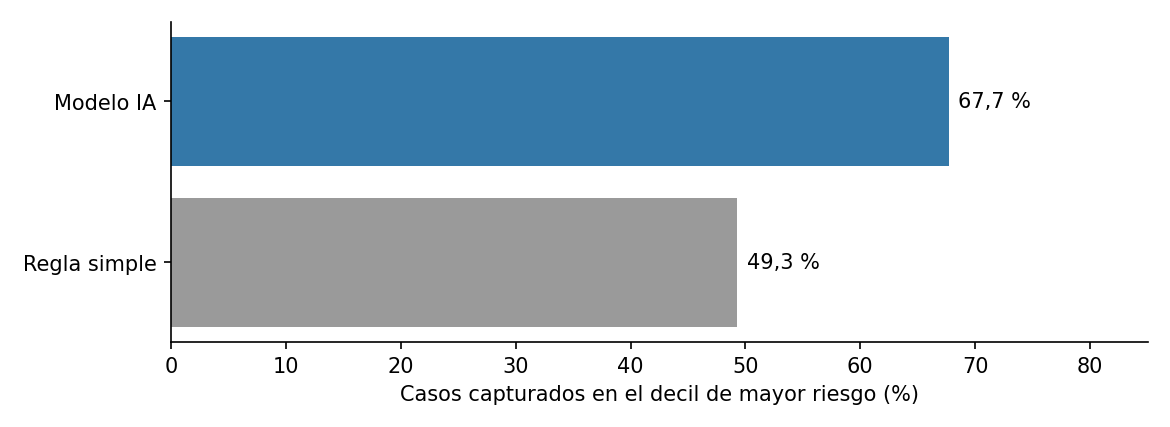
\includegraphics[width=0.62\textwidth]{fig5_oxigenodependencia.png}
\caption{Concentración de casos de oxigenodependencia a tres meses en el 10~\% de niños con mayor riesgo; cifras internas reportadas.}
\label{fig:oxigeno}
\end{figure}

\textbf{Detección de anomalías.} La evaluación del detector inyectó seis clases de errores en la partición de prueba: códigos, unidades, desviaciones de tres desviaciones estándar, dígitos invertidos, intercambio de etapas y valores procedentes de otro niño (Fig.~\ref{fig:deteccion}). La detección global documentada fue del 75,3~\% con 18,8 alertas por cada 1.000 registros sin perturbación inyectada, frente a 14,7 alertas de la regla vigente. La ganancia fue especialmente marcada en desviaciones de tres DE (78~\% frente a 27~\%) y etapas intercambiadas (68~\% frente a 5~\%); los valores de otro niño fueron los más difíciles de identificar (34~\%). Estas cifras describen escenarios de prueba específicos y no la sensibilidad ante todos los errores reales.

\begin{figure}[!htb]
\centering
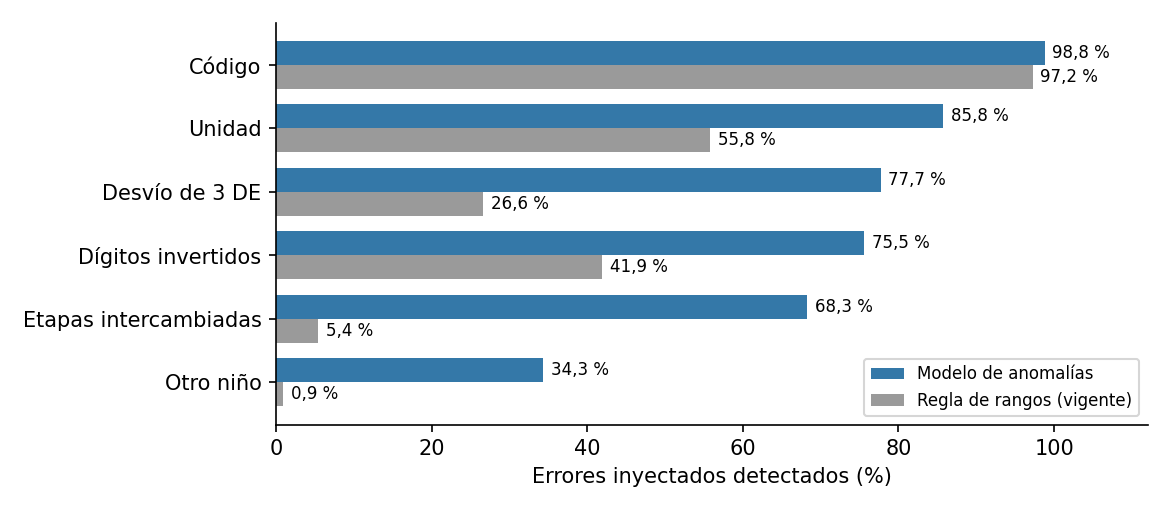
\includegraphics[width=0.72\textwidth]{fig4_deteccion.png}
\caption{Porcentaje de errores inyectados detectados por tipo en la partición de prueba: modelo de anomalías frente a la regla de rangos vigente.}
\label{fig:deteccion}
\end{figure}

\textbf{Calidad de datos.} Se identificaron además 33 fechas imposibles, 985 eventos fechados antes del parto y 5.905 registros de crecimiento con edad distinta a la de la visita. Estos hallazgos apoyan el valor del control de calidad antes del modelamiento, pero requieren confirmación y depuración en origen.

\section{ANÁLISIS DE LOS RESULTADOS OBTENIDOS, RETOS Y CÓMO PROSEGUIR}

La lectura conjunta de AUC y calibración es esencial: un clasificador puede ordenar mejor el riesgo y simultáneamente sobreestimar probabilidades. Las métricas de la Tabla~\ref{tab:validacion} describen discriminación en prueba retrospectiva; no equivalen a sensibilidad clínica en un umbral específico ni prueban utilidad prospectiva, y deben completarse con prevalencia, AUC-PR, intervalos de confianza y curvas de calibración.

\textbf{Sobreestimación en readmisión.} La sobreestimación no se limita a oxigenodependencia: las cinco ventanas de readmisión presentan razones riesgo/observado entre 1,39 y 2,96 (máxima en 3--6 meses), con prevalencias bajas (1,57--4,90~\%). Además, en dos de ellas (40 semanas--3 meses y 3--6 meses) la regla simple concentra más casos en el decil superior que el modelo (23,1 frente a 22,4~\% y 18,5 frente a 16,7~\%), pese a tener menor AUC. Una explicación plausible, que debe verificarse, es que la calibración isotónica no se traslada bien entre periodos con distinta prevalencia, en línea con el aumento de readmisiones registrado desde 2021, que aún se revisa para distinguir variación clínica de cambio de codificación. Por ello, la recalibración por periodo es prioritaria antes de fijar umbrales. En contraste, los desenlaces de inasistencia están razonablemente calibrados (0,84--1,06) pero discriminan poco (AUC de 0,56 a 0,67), por lo que su utilidad operativa debe evaluarse con precisión-recall.

Posterior a la revisión de los resultados observados en los 14 desenlaces, el equipo sostuvo una sesión con el experto que acompaña el proyecto, quien sugirió enfocar el trabajo en dos o tres desenlaces puntuales. Esta recomendación orienta la siguiente fase: en lugar de distribuir el esfuerzo entre todas las ventanas evaluadas, se priorizará un número reducido de desenlaces para profundizar en su definición, calibración, análisis de incertidumbre y utilidad clínica. Para esos desenlaces se incorporarán los resultados de explicabilidad (importancia global TreeSHAP y ejemplos individuales revisados por clínicos), que este avance aún no presenta.

La mejora frente a reglas simples indica que el contexto del niño y su trayectoria contienen información útil que las verificaciones aisladas no capturan. No obstante, la evaluación con perturbaciones artificiales puede sobreestimar la detección de errores naturales y un AUROC elevado no garantiza una carga de alertas aceptable. La revisión humana y la evaluación de calibración por subgrupos son necesarias antes de cualquier uso asistencial.

La pérdida de seguimiento es un riesgo metodológico central (Sección 2.2). Exigir las 18 mediciones de peso, talla y perímetro cefálico en seis visitas generaría una cohorte altamente seleccionada que favorecería a los pacientes con mejor adherencia; por ello, ese subconjunto completo se reservará para análisis de sensibilidad y caracterización de trayectorias, mientras que los clasificadores incrementales utilizarán la información disponible hasta cada corte y documentarán los patrones de ausencia.

El quiebre de registro de 2022 constituye una amenaza de deriva: los pesos redondeados a 100 g aumentaron del 0,9~\% al 5,4~\%, y las diferencias de prácticas de medición pueden confundirse con cambios biológicos. Ello obliga a controlar quiebres históricos, verificar estabilidad de unidades y validar temporalmente en cohortes posteriores. También quedan por consolidar el diccionario de variables, las referencias de crecimiento según edad y población, la definición de algunos desenlaces y el manejo de mediciones registradas fuera de ventana.

Como continuación se propone en el desarrollo de este proyecto:
\begin{enumerate}[label=(\roman*),leftmargin=*,itemsep=0pt,topsep=0pt]
\item congelar el corte y la versión del diccionario para reproducir métricas;
\item completar la auditoría por desenlace y subgrupo, con curvas de calibración, intervalos de confianza, AUC-PR y recalibración por periodo;
\item implementar las firmas incrementales en 40 semanas, 3, 6 y 9 meses para predicción a 12 meses, comparando una línea base perinatal, un modelo con estado antropométrico actual y otro con cambios longitudinales acumulados; solo la diferencia entre estos dos últimos cuantifica el aporte específico de la trayectoria;
\item revisar con expertos una muestra ciega de anomalías, alertas y explicaciones individuales, que no se interpretarán como evidencia causal; y
\item contrastar las predicciones emitidas con el corte del 24 de julio de 2026 frente a una carga posterior de la Fundación, cuando esté disponible, respetando el tiempo de maduración de cada desenlace y sin presentarlo como validación concluida hasta disponer de los resultados observados.
\end{enumerate}

La plataforma debe conservar umbrales configurables, registro de versiones y separación entre datos reales y simulados.

\renewcommand{\refname}{REFERENCIAS}
\begin{thebibliography}{99}
\bibitem{charpak2005} N. Charpak et al., ``Kangaroo Mother Care: 25 years after,'' \emph{Acta Paediatrica}, vol. 94, no. 5, pp. 514--522, 2005, doi: 10.1111/j.1651-2227.2005.tb01930.x.
\bibitem{who2022} World Health Organization, \emph{WHO Recommendations for Care of the Preterm or Low-Birth-Weight Infant}. Geneva, Switzerland: WHO, 2022.
\bibitem{ke2017} G. Ke et al., ``LightGBM: A highly efficient gradient boosting decision tree,'' in \emph{Advances in Neural Information Processing Systems}, vol. 30, 2017.
\bibitem{angelopoulos2023} A. N. Angelopoulos and S. Bates, ``Conformal prediction: A gentle introduction,'' \emph{Foundations and Trends in Machine Learning}, vol. 16, no. 4, pp. 494--591, 2023, doi: 10.1561/2200000101.
\bibitem{page1954} E. S. Page, ``Continuous inspection schemes,'' \emph{Biometrika}, vol. 41, no. 1/2, pp. 100--115, 1954, doi: 10.1093/biomet/41.1-2.100.
\bibitem{zadrozny2002} B. Zadrozny and C. Elkan, ``Transforming classifier scores into accurate multiclass probability estimates,'' in \emph{Proc. 8th ACM SIGKDD Int. Conf. Knowledge Discovery and Data Mining}, 2002, pp. 694--699, doi: 10.1145/775047.775151.
\bibitem{lundberg2017} S. M. Lundberg and S.-I. Lee, ``A unified approach to interpreting model predictions,'' in \emph{Advances in Neural Information Processing Systems}, vol. 30, 2017.
\bibitem{lundberg2020} S. M. Lundberg et al., ``From local explanations to global understanding with explainable AI for trees,'' \emph{Nature Machine Intelligence}, vol. 2, no. 1, pp. 56--67, 2020, doi: 10.1038/s42256-019-0138-9.
\bibitem{villar2015} J. Villar et al., ``Postnatal growth standards for preterm infants,'' \emph{The Lancet Global Health}, vol. 3, no. 11, pp. e681--e691, 2015, doi: 10.1016/S2214-109X(15)00163-1.
\bibitem{fenton2013} T. R. Fenton and J. H. Kim, ``A systematic review and meta-analysis to revise the Fenton growth chart for preterm infants,'' \emph{BMC Pediatrics}, vol. 13, art. 59, 2013, doi: 10.1186/1471-2431-13-59.
\bibitem{collins2024} G. S. Collins et al., ``TRIPOD+AI statement: updated guidance for reporting clinical prediction models that use regression or machine learning methods,'' \emph{BMJ}, vol. 385, e078378, 2024, doi: 10.1136/bmj-2023-078378.
\end{thebibliography}

\end{document}
